% ICCV 2025 Paper Template

\documentclass[10pt,twocolumn,letterpaper]{article}

%%%%%%%%% PAPER TYPE  - PLEASE UPDATE FOR FINAL VERSION
% \usepackage{iccv}              % To produce the CAMERA-READY version
%\usepackage[review]{iccv}      % To produce the REVIEW version
\usepackage[pagenumbers]{iccv} % To force page numbers, e.g. for an arXiv version

% Import additional packages in the preamble file, before hyperref
%
% --- inline annotations
%
\newcommand{\red}[1]{{\color{red}#1}}
\newcommand{\todo}[1]{{\color{red}#1}}
\newcommand{\TODO}[1]{\textbf{\color{red}[TODO: #1]}}
% --- disable by uncommenting  
% \renewcommand{\TODO}[1]{}
% \renewcommand{\todo}[1]{#1}
\usepackage{graphicx}
\usepackage{booktabs}
\usepackage{multirow}
\usepackage{longtable}
\usepackage{comment}
\usepackage{placeins}
\usepackage{graphicx}
\usepackage{titletoc}
\usepackage{tabularx}
\usepackage{amsmath}
\usepackage{float}
\usepackage[accsupp]{axessibility}  % Improves PDF readability for those with disabilities.

\usepackage{adjustbox}
\usepackage{tikz} % Fig. in sections/method.tex
\usetikzlibrary{arrows.meta,shadows}

% It is strongly recommended to use hyperref, especially for the review version.
% hyperref with option pagebackref eases the reviewers' job.
% Please disable hyperref *only* if you encounter grave issues, 
% e.g. with the file validation for the camera-ready version.
%
% If you comment hyperref and then uncomment it, you should delete *.aux before re-running LaTeX.
% (Or just hit 'q' on the first LaTeX run, let it finish, and you should be clear).
\definecolor{iccvblue}{rgb}{0.21,0.49,0.74}
\usepackage[pagebackref,breaklinks,colorlinks,allcolors=iccvblue]{hyperref}

%%%%%%%%% PAPER ID  - PLEASE UPDATE
\def\paperID{8610} % *** Enter the Paper ID here
\def\confName{ICCV}
\def\confYear{2025}

%%%%%%%%% TITLE - PLEASE UPDATE
\title{
ISLES 2024 Stroke lesion segmentation
}
%%%%%%%%% AUTHORS - PLEASE UPDATE
\author{Raiyaan Abdullah\\
%Center for Research in Computer Vision\\
%University of Central Florida\\
{\tt\small ra164195@ucf.edu}
% For a paper whose authors are all at the same institution,
% omit the following lines up until the closing ``}''.
% Additional authors and addresses can be added with ``\and'',
% just like the second author.
% To save space, use either the email address or home page, not both
\and
NID: 5566965\\
%Center for Vision Technology,\\
%SRI International, Princeton\\
% For a paper whose authors are all at the same institution,
% omit the following lines up until the closing ``}''.
% Additional authors and addresses can be added with ``\and'',
% just like the second author.
% To save space, use either the email address or home page, not both
}

\begin{document}
\maketitle
\begin{abstract}

\end{abstract}

\section{Problem and motivation}


\section{Related Work and Research Gap}
\label{rel}

ISLES'24 is different from most stroke lesion segmentation benchmarks. The goal is not to segment a lesion that is already visible in the scan. Instead, the model has to predict the final, post-treatment infarct using only images taken before treatment. The challenge provides acute multimodal CT scans (NCCT, CTA, native 4D CTP, and derived perfusion maps) along with clinical information, while the ground truth infarct is drawn from a follow-up MRI~\cite{delarosa2024isles24,riedel2026isles24dataset}. This makes the task closer to predicting a patient-specific outcome than to standard lesion segmentation.

Results from the ISLES'24 challenge show that nnU-Net is a strong baseline, but preprocessing and modality choice matter just as much as the architecture. All three top teams used a variant of nnU-Net. The winning team, Kurtlab, combined a large residual-encoder 3D nnU-Net with skull stripping and custom intensity windowing, reaching a mean test Dice of about 0.285. The second-place team, AMC-Axolotls, used a cascaded nnU-Net. The third-place team, Ninjas, got competitive results using only the native 4D CTP sequence~\cite{delarosa2024isles24,ren2025isles24}. Ren et al. showed that this kind of clinically motivated preprocessing gave a large boost over the default nnU-Net pipeline~\cite{ren2025isles24}. More recently, Martinez Cegarra et al. compared a single-stage nnU-Net, a cascaded nnU-Net, and a transformer-based model (SegFormer3D) on the same data split and preprocessing setup. The convolutional models were still hard to beat in this low-data setting, though the authors note that some framework-specific training choices make a fully fair architecture comparison difficult~\cite{cegarra2026isles}.

Work on stroke outcome prediction before ISLES'24 also supports using the temporal information in CTP instead of only relying on derived perfusion maps. Robben et al. predicted the final infarct directly from native CTP scans plus treatment and timing information, and found through an ablation study that native CTP gave better predictions than deconvolved perfusion maps~\cite{robben2020nativectp}. Building on this, Amador et al. designed a spatio-temporal network that processes the full 4D CTP sequence directly. Their model reached a mean Dice of 0.45, compared to 0.38 for a perfusion-map baseline, which supports modeling both the spatial and temporal dimensions of perfusion data~\cite{amador2022spatiotemporal}.

These results leave an open question for ISLES'24. Once a strong, consistently preprocessed segmentation baseline is in place, it is still not clear how much extra information different acute imaging inputs and clinical variables actually add. A controlled comparison, or a multimodal extension that keeps the same data split, preprocessing, and evaluation protocol, could show whether extra temporal or clinical information genuinely improves final infarct prediction, rather than the gains simply coming from a different architecture.

% Sections 4-5 (Jahid). Switch to another method file here when that version exists.
% Sections 4 (Proposed method) and 5 (Dataset and experiments) -- Jahid
% Version 1: in line with the current Novelty section (perfusion maps presented to a video encoder as an ordered sequence).

\section{Proposed method}
\label{sec:method}

\begin{figure}[t]
\centering
\resizebox{\columnwidth}{!}{%
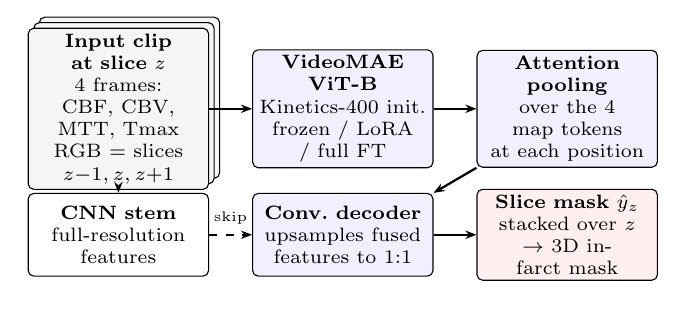
\begin{tikzpicture}[
  box/.style={draw, rounded corners=2pt, align=center, font=\scriptsize, minimum height=1.05cm, text width=2.15cm, inner sep=2pt},
  inclip/.style={box, fill=gray!8, double copy shadow={shadow xshift=2pt, shadow yshift=2pt, fill=gray!8, draw}},
  arr/.style={-{Stealth[length=4pt]}, thick},
  skip/.style={-{Stealth[length=4pt]}, thick, dashed}]
  \node[inclip] (in) at (0,0) {\textbf{Input clip at slice $z$}\\4 frames: CBF, CBV, MTT, Tmax\\RGB $=$ slices $z{-}1, z, z{+}1$};
  \node[box, fill=blue!6] (enc) at (2.85,0) {\textbf{VideoMAE ViT-B}\\Kinetics-400 init.\\frozen / LoRA / full FT};
  \node[box, fill=blue!6] (pool) at (5.7,0) {\textbf{Attention pooling}\\over the 4 map tokens\\at each position};
  \node[box] (stem) at (0,-1.6) {\textbf{CNN stem}\\full-resolution\\features};
  \node[box, fill=blue!6] (dec) at (2.85,-1.6) {\textbf{Conv.\ decoder}\\upsamples fused\\features to 1:1};
  \node[box, fill=red!6] (out) at (5.7,-1.6) {\textbf{Slice mask $\hat{y}_z$}\\stacked over $z$\\$\rightarrow$ 3D infarct mask};
  \draw[arr] (in) -- (enc);
  \draw[arr] (enc) -- (pool);
  \draw[arr] (pool.south west) -- (dec.north east);
  \draw[arr] (in) -- (stem);
  \draw[skip] (stem) -- node[above, font=\tiny]{skip} (dec);
  \draw[arr] (dec) -- (out);
\end{tikzpicture}}
\caption{Perfusion-as-video model. The four perfusion maps form the time axis of a short clip, so the video encoder models relations \emph{between} maps instead of mixing them as input channels.}
\label{fig:method}
\end{figure}

\paragraph{Shared preprocessing and baseline.}
All models use the organisers' co-registered images~\cite{delarosa2024isles24} and the preprocessing of the winning ISLES'24 entry. That pipeline applies SynthStrip skull stripping to the NCCT, propagates the mask to the other scans, and clips each input to a fixed window: CTA 0--90\,HU, CBF 0--35\,mL/100\,g/min, CBV 0--10\,mL/100\,g, MTT 0--20\,s and Tmax 0--7\,s~\cite{ren2025isles24}. The baseline is the same 3D full-resolution nnU-Net with the large residual encoder (ResEnc L) that won the challenge, with the inputs stacked as channels~\cite{ren2025isles24,isensee2024revisited}.

\paragraph{Perfusion-as-video model.}
Instead of stacking the perfusion maps as channels, we present them to a video encoder as an ordered clip (Fig.~\ref{fig:method}). For each axial slice $z$, the clip has four frames in a fixed order: CBF, CBV, MTT, Tmax. The three colour channels of each frame hold slices $z{-}1$, $z$ and $z{+}1$ of that map. This gives 2.5D context and matches the pretrained input format. The encoder is a ViT-B VideoMAE pretrained on Kinetics-400~\cite{tong2022videomae}. We chose it because VideoMAE learns well from very small video datasets. VideoMAE embeds $2{\times}16{\times}16$ space-time cubes~\cite{tong2022videomae}, so we repeat each map twice. Every cube then covers exactly one map, and the pretrained embedding is reused unchanged. A learned attention-pooling layer fuses the four map tokens at each spatial position. A convolutional decoder then upsamples the fused features to a per-slice infarct probability. The ViT works at 1/16 resolution, and small infarcts are where every ISLES'24 method struggled~\cite{delarosa2024isles24}, so the decoder also receives skip features from a light CNN stem applied to the full-resolution input. Slice predictions are stacked into a 3D mask. Training uses Dice plus cross-entropy loss, as in the top challenge entries~\cite{delarosa2024isles24}.

\paragraph{Adaptation.}
With only 149 training cases, we compare three ways of adapting the pretrained encoder:
\begin{enumerate*}[label=(\roman*)]
  \item freezing it, and training only the pooling layer and decoder;
  \item LoRA, which keeps the pretrained weights frozen and trains low-rank updates in the attention layers~\cite{hu2022lora};
  \item full fine-tuning.
\end{enumerate*}
Natural-video pretraining has improved 3D models on chest CT detection tasks~\cite{ke2023videopretraining}. Whether it also transfers to perfusion maps is part of what we test.

\section{Dataset and experiments}
\label{sec:experiments}

\paragraph{Data and splits.}
We use the 149 public ISLES'24 training cases from two centres. The 96-case test set is hidden~\cite{riedel2026isles24dataset}. The labels are infarct masks drawn on follow-up MRI acquired 2--9 days after treatment~\cite{riedel2026isles24dataset}. Only patients with successful recanalisation (TICI 2b/3) are included~\cite{delarosa2024isles24}. We run 5-fold cross-validation, with folds stratified by centre and by lesion volume ($<$5 vs.\ $\geq$5\,mL). Every method uses identical folds. Checkpoints and hyperparameters are chosen on a validation split inside each training fold, so the 149 out-of-fold predictions are never used for tuning.

\paragraph{Baselines and metrics.}
\begin{enumerate*}[label=(B\arabic*), start=0]
  \item the clinical rCBF\,$<$\,30\% threshold, a baseline in the challenge itself~\cite{delarosa2024isles24};
  \item our reproduction of nnU-Net ResEnc L on the same four maps as our model;
  \item the same nnU-Net with CTA added, as in the winning configuration~\cite{ren2025isles24}.
\end{enumerate*}
The challenge's best hidden-test Dice of 0.285~\cite{delarosa2024isles24} is quoted for context only, because it comes from a different test set. We report the four challenge metrics using the official evaluation code: Dice, absolute volume difference (mL), lesion-wise F1 and absolute lesion count difference~\cite{delarosa2024isles24}. Each metric is reported overall, for infarcts under 5\,mL, and for each centre.

\paragraph{Principal comparison and ablations.}
The main comparison is B1 against the video model on identical inputs. We test it with a paired Wilcoxon signed-rank test on per-case Dice. Five ablations locate the source of any difference:
\begin{enumerate*}[label=(A\arabic*)]
  \item the same backbone with the maps fused as channels of a single frame, instead of as separate frames;
  \item map order shuffled during training and testing, to test whether order carries information;
  \item Kinetics initialisation vs.\ random initialisation;
  \item frozen vs.\ LoRA vs.\ full fine-tuning;
  \item NCCT and CTA added as extra frames.
\end{enumerate*}
If the video model only matches B1 when the order is shuffled (A2) or when the maps are fused as channels (A1), its benefit comes from pretraining rather than from sequence modelling.


\section{Novelty}
\label{nov}
Existing work on ISLES'24 has largely relied on nnU-Net-based architectures. After establishing a strong nnU-Net baseline, I want to investigate how alternative model families perform under the same preprocessing, data split, and evaluation protocol. I am particularly interested in video-encoder architectures, because there is a useful structural analogy between their inputs and multimodal perfusion imaging. In the standard ISLES'24 setting, nnU-Net receives several aligned 3D volumes, such as CBF, CBV, MTT, and Tmax, stacked as input channels. Video models, in contrast, are designed to extract information from ordered stacks of 2D frames while modeling relationships across the additional dimension.

This motivates exploring whether video encoders can be adapted to exploit the relationships between perfusion maps more effectively than treating them simply as independent channels of a 3D segmentation network. For example, the perfusion maps could be represented as an ordered sequence or processed using a video backbone with a task-specific fusion mechanism, followed by a segmentation decoder that reconstructs a 3D infarct prediction. The goal would not simply be to replace nnU-Net, but to determine whether architectures designed to model relationships across sequences can provide a useful inductive bias for multimodal perfusion imaging and improve final infarct prediction.

\section{Feasibility and fallback plan}
The ISLES'24 public release contains 149 training cases, while the official 96-case test set remains hidden and is no longer available for routine post-challenge submissions. Therefore, we will evaluate all models using the publicly available cohort, either through a fixed held-out test split or, preferably, cross-validation with identical folds across all methods. This will allow a fair comparison between the nnU-Net baseline and alternative architectures while keeping the data split, preprocessing, and evaluation protocol consistent. Training modern video-based encoders can be computationally expensive, particularly when adapting them to volumetric medical imaging, so experiments will be designed to fit within approximately 48 GB of GPU memory by adjusting model size, batch size, input resolution, and sampling strategy where needed. Training will be carried out using the Newton computing cluster and available laboratory GPUs.

Reproducing the nnU-Net baseline is expected to be relatively low risk because the framework is mature and has already been extensively used on ISLES'24. The main technical risk lies in adapting video architectures to perfusion imaging, since CBF, CBV, MTT, and Tmax are distinct physiological maps rather than true temporal video frames. A video-style encoder may therefore fail to provide a useful inductive bias and could underperform the nnU-Net baseline. If this occurs, the study will focus on analyzing why the adaptation fails, including whether the limitation arises from modality representation, ordering, data scarcity, spatial inconsistency, or the architecture itself. Such negative results would still help clarify whether video-based encoders are suitable for derived perfusion maps and whether they may instead be better suited to native 4D CTP data, where a genuine temporal dimension is present.   

{\small
\bibliographystyle{ieeenat_fullname}
\bibliography{main}
}
\end{document}
